% CVPR 2022 Paper Template
% based on the CVPR template provided by Ming-Ming Cheng (https://github.com/MCG-NKU/CVPR_Template)
% modified and extended by Stefan Roth (stefan.roth@NOSPAMtu-darmstadt.de)

\documentclass[10pt,twocolumn,letterpaper]{article}

%%%%%%%%% PAPER TYPE  - PLEASE UPDATE FOR FINAL VERSION
%\usepackage[review]{cvpr}      % To produce the REVIEW version
\usepackage{cvpr}              % To produce the CAMERA-READY version
%\usepackage[pagenumbers]{cvpr} % To force page numbers, e.g. for an arXiv version

% Include other packages here, before hyperref.
\usepackage{graphicx}
\usepackage{amsmath}
\usepackage{amssymb}
\usepackage{booktabs}


% It is strongly recommended to use hyperref, especially for the review version.
% hyperref with option pagebackref eases the reviewers' job.
% Please disable hyperref *only* if you encounter grave issues, e.g. with the
% file validation for the camera-ready version.
%
% If you comment hyperref and then uncomment it, you should delete
% ReviewTempalte.aux before re-running LaTeX.
% (Or just hit 'q' on the first LaTeX run, let it finish, and you
%  should be clear).
\usepackage[pagebackref,breaklinks,colorlinks]{hyperref}


% Support for easy cross-referencing
\usepackage[capitalize]{cleveref}
\crefname{section}{Sec.}{Secs.}
\Crefname{section}{Section}{Sections}
\Crefname{table}{Table}{Tables}
\crefname{table}{Tab.}{Tabs.}


%%%%%%%%% PAPER ID  - PLEASE UPDATE
\def\cvprPaperID{*****} % *** Enter the CVPR Paper ID here
\def\confName{CVPR}
\def\confYear{2022}


\begin{document}

%%%%%%%%% TITLE - PLEASE UPDATE
\title{Open-Set Domain Adaptation through Self-Supervision}

\author{Daniele Rege Cambrin, Kylie Bedwell, Tommaso Natta, Ehsan Ansari Nejad\\
Politecnico di Torino\\
Corso Duca degli Abruzzi, 24\\
10129 Torino, ITALY\\
{\tt\small s290144@studenti.polito.it, s287581@studenti.polito.it} \\
{\tt\small s282478@studenti.polito.it, s288903@studenti.polito.it}
% For a paper whose authors are all at the same institution,
% omit the following lines up until the closing ``}''.
% Additional authors and addresses can be added with ``\and'',
% just like the second author.
% To save space, use either the email address or home page, not both
}
\maketitle

%%%%%%%%% ABSTRACT
\begin{abstract}
   - sentence describing the problem
 - sentence describing our proposed method
 - sentence summarising the results
 - sentence about the variations
 - sentence about the variation results
\end{abstract}

%%%%%%%%% BODY TEXT
\section{Introduction}
\label{sec:intro}

In the computer vision research area large amounts of unlabeled data are available, however the cost of labeling this data is high ~\cite{Csurka2017, Zhang2016}. Domain adaptation is one technique that can be used to exploit the unlabeled data by first training a model on labeled data from a different but similar domain (the \textit{source} domain), and then applying this model to the unlabeled data ( the \textit{target} domain). This technique assumes the distribution of both source and target domains are similar and describe the same class labels, also known as the \textit{closed-set} scenario~\cite{Bucci2020}. When applied to real-word scenarios however it is possible that the target domain includes previously unseen classes, known as the \textit{open-set} scenario. These extra class labels in the target domain will cause performance degradation of the classification model and should be identified and isolated. The problem thus consists of two steps: first separating the target domain into known and unknown samples; then conducting domain alignment between the source domain and the known samples of the target domain. 

Self-supervised learning can be used to separate the known class samples in the target domain from the unknown samples. Self-supervised learning involves the transformation of data using a known transform (for example by using image rotation), then training a model to predict the transformation~\cite{Xu2019}. When used in an object classification task and considering the image rotation transformation, the correct orientation of an object is domain-invariant. In this way the model can be trained to predict the correct orientation of the image using data from the source domain, then applied to the images of the target domain. If the orientation of a sample in the target domain is predicted correctly then it is considered to be of a \textit{known} class. Contrarily if the orientation is not prediction correctly it is labelled as \textit{unknown}. 

Domain adaptation can then be performed between the samples in the source domain and the samples recognized as known in the target domain. When applying domain adaptation to an open-set scenario (Open-Set Domain Adapatation or OSDA) the samples classified as unknown can be treated as a separate class and incorporated into the Closed-Set Domain Adaptation (CSDA) task~\cite{Pau2020}. The self-supervised rotation task can also be used to reduce the domain shift during this step, using the Rotation-based Open Set (ROS) method developed by Bucci \etal \cite{Bucci2020}.

This study investigates the use of a simplified ROS method for object classification on the \textit{Office-Home} dataset \cite{OfficeHome}. Alternative self-supervised tasks \textcolor{red}{as well as the inclusion of center-loss} are also considered and their performance on the object classification task is evaluated.


%------------------------------------------------------------------------
\section{Related Work}
\label{sec:relatedWork}

\textbf{Anomaly detection}, or outlier/novelty detection, in an open-set scenario can be used to detect samples belonging to the unknown or unseen class. Various different approaches for anomaly detection have been used in the literature as applied to the open-set scenario. Golan and El-Yanic \cite{Golan2018} present a method for using geometric transformations to create a self-labeled dataset. In this way the neural classifier learns features that are effective for the detection of anomalies.  Sakurada and Yairi \cite{Sakurada2014} on the other hand make use of autoencoders with dimensionality reduction. This method assumes the data have correlations that can clearly separate normal and anomalous samples when reduced to a lower dimensional subspace. After the test data is projected into the subspace it is then reconstructed and the corresponding reconstruction error is used to identify the anomalous samples.


\textbf{Self-supervised learning} has been a key concept aimed at reducing the need for human labeling of data. It has also created opportunities for the use of data in problems where supervision is not possible \cite{Yaman2020}. Self-supervised learning consists of choosing a self-supervised task (or pretext task) to train alongside the main classification task. One possible self-supervised task is image rotation prediction, which is reported to perform best for visual representation learning \cite{Xu2019, Gidaris2018}. However many options are available, including image-patch based methods \cite{Mundhenk2018, Kim2018}, horizontal flipping \cite{Golan2018}, or by solving jigsaw puzzles \cite{Carlucci2019, Kim2018}. 


\textbf{Domain adaptation} techniques have advanced significantly in recent years for the closed-set scenario \cite{Pau2020}, however for real-world applications the closed-set assumption is often not applicable \cite{Ren2021}. It has become increasingly important to develop robust techniques for open-set domain adaptation to address this problem. Recent studies in this field include: the development of a generic approach to learn a linear mapping between the features of the source domain and target domain \cite{Pau2020}; the use of self-supervision to improve the generalization of models to different domains \cite{Carlucci2019}; partial domain adaptation by using a discrepancy criterion to partially align features whilst avoiding negative transfer \cite{Ren2021}. These techniques have been reported to perform well, and increase the applicability of domain adaptation methods to real-world applications \cite{Carlucci2019, Ren2021,Pau2020}.


\textbf{Rotation-based Open Set} (ROS) is a specific technique developed by Bucci \etal \cite{Bucci2020}. ROS is a two-stage method for open-set domain adaptation. The first stage separates samples in the target domain into known and unknown categories by training the model on a multi-rotation recognition task. The rotation recognition task includes the use of the center-loss to improve performance by learning a center of the features and minimizing the distances between features and their corresponding centers \cite{Wen2016}. The second stage conducts domain alignment, training both semantic and rotation classifiers to classify known target samples. Bucci \etal \cite{Bucci2020} also propose the use of the harmonic mean of the average class accuracies  for the known and unknown classes as a more robust and balanced evaluation metric.


%------------------------------------------------------------------------
\section{Method}
\label{sec:method}

This study aims to solve the open-set scenario by using self-supervised learning with domain adaptation. Image rotation recognition has been chosen as the self-supervised task due to it's good performance for visual representation learning \cite{Xu2019, Gidaris2018}. The rotation recognition task involves taking the original image sample from the source domain and rotating it clockwise a set amount (for example by 0$^{\circ}$, 90$^{\circ}$, 180$^{\circ}$ or 270$^{\circ}$). A rotation classifier is then trained to predict the correct orientation of the object. The correct orientation of the object, however, is not an inherent property of an image, for example consider the pens in Figure \ref{fig:RotatedPens}. When analysing a rotated image of a pen it is not possible to infer the original rotation. The original image is therefore included in the rotation classifier and the relative rotation analysed instead. In training the rotation classifier the features of the original sample are concatenated with the features of the rotated sample. By including the original samples the network is also able to learn features that are more discriminative between class labels, focussing more on the shape of the object and less on the texture \cite{Bucci2020}, as shown in Figure \ref{fig:RotationFeatures}.

\begin{figure}[!htb]
  \centering
   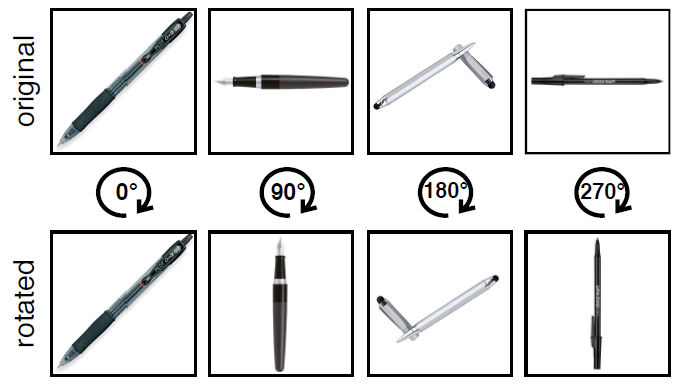
\includegraphics[width=0.9\linewidth]{Figures/RotatedPens.png}
   \caption{Relative orientations of pens with respect to the original images \cite{Bucci2020}.}
   \label{fig:RotatedPens}
\end{figure}

\begin{figure}[!htb]
  \centering
   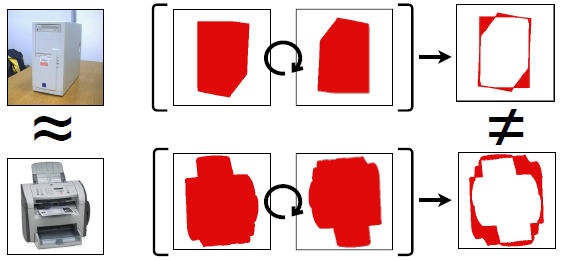
\includegraphics[width=0.9\linewidth]{Figures/RotationFeatures.png}
   \caption{Image rotations help the network learn features that discriminate the shape of objects \cite{Bucci2020}.}
   \label{fig:RotationFeatures}
\end{figure}

To solve the open-set domain adaptation problem a simplified version of the ROS method (Figure \ref{fig:ROS}) is used. This version uses a single-head rotation classifier and does not include the center-loss, \textcolor{red}{however the effect of the center-loss is evaluated subsequently as a variation to this method}. Alternative self-supervised tasks are also considered, including horizontal flipping, \textcolor{red}{vertical flipping} and through solving jigsaw puzzles. These variations are analyzed in Section \ref{sec:variations}.

\begin{figure*}[!htb]
  \centering
   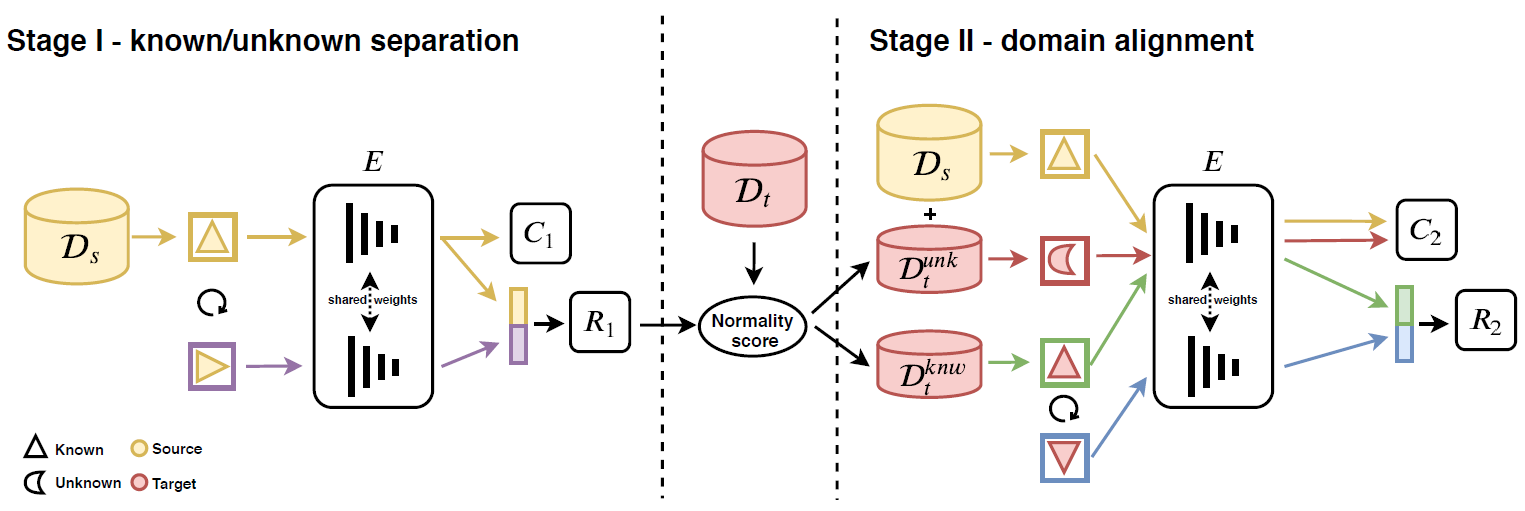
\includegraphics[width=0.9\linewidth]{Figures/ROS.png}
   \caption{Rotation-based Open Set (ROS) method schematic illustration \cite{Bucci2020}.}
   \label{fig:ROS}
\end{figure*}

\subsection{Stage I - known/unknown separation}

Stage I of the simplified ROS method involves training both an object classifier and a rotation recognition task on data from the source domain, as shown on the left side of Figure \ref{fig:ROS}, where $D_S$ is the source domain dataset, $E$ is the encoder, $C_1$ is the object classifier and $R_1$ is the rotation classifier. The object prediction is based on the features of the original source samples, whereas the rotation prediction is based on the concatenated features of the original and rotated samples. The object classification and rotation recognition tasks are trained simultaneously to minimize the total loss objective function given by:
\begin{equation}
  L_{tot} = L_{cls} + \alpha_1 L_{rot} ,
  \label{eq:totalloss}
\end{equation}
where $L_{cls}$ is the loss from the object classifier, $L_{rot}$ is the loss from the rotation classifier, and $\alpha_1$ is the weight assigned to the rotation recognition task. The value of $\alpha_1$ is tuned according to the performance of the network, as detailed in Section \ref{sec:ablation}.


\subsection{Target evaluation}

\subsection{Stage II - domain alignment}

\subsection{Final evaluation}

- describe in detail the method used
- include the diagrams here and explain them
- explain the evaluation parameters that will be used

%------------------------------------------------------------------------
\section{Experiments}
\label{sec:experiments}

\subsection{Ablation study}
\label{sec:ablation}

\subsection{Results}

- the network used
- ablation study: hyperparameter tuning of weights and threshold value, include graphs or tables of values


%------------------------------------------------------------------------
\section{Variations}
\label{sec:variations}

- describe each of the variations
- present results of the performance of the model and compare with the baseline for each of the variations

%------------------------------------------------------------------------
\section{Conclusions}
\label{sec:conclusion}

- summarise the results
- add future recommendations

\subsection{Acknowledgements}
The authors would like to thank Silvia Bucci for her assistance and guidance in completing this study.


%%%%%%%%% REFERENCES
{\small
\bibliographystyle{ieee_fullname}
\bibliography{egbib}
}

\end{document}
